% Section content template for individual Educative lessons
% This file contains the actual content for a specific section
% Generated from Educative API section content

% Section: High-level Design of Uber
% Section ID: 5429357153091584
% Section Slug: high-level-design-of-uber
% Generated: 2025-12-07T23:31:12.044731

\subsection{Workflow of our application}\label{Z4oMYGyfgAdPaK3vHlVDs}
\\
Before diving deep into the design, let's understand how our application works. The following steps show the workflow of our application:

\begin{enumerate}
\item
\protect\phantomsection\label{ka24GPAxr-5JZPhmjOotw}
All the nearby drivers except those already serving rides can be seen when the rider starts our application.
\item
\protect\phantomsection\label{TPMRcOuGgT-GMiyVIhEY0}
The rider enters the drop-off location and requests a ride.
\item
\protect\phantomsection\label{zBU3pbuC4El78naUseSKL}
The application receives the request and finds a suitable driver.
\item
\protect\phantomsection\label{SgyfwTvs3251Y7BXRRTVS}
Until a matching driver is found, the status will be ``Waiting for the driver to respond.''
\item
\protect\phantomsection\label{mhS-UAjDyEi4zc8PJxNi9}
The drivers report their location every four seconds. The application finds the trip information and returns it to the driver.
\item
\protect\phantomsection\label{_S9OYlgkBpdmKLnbGyFZA}
The driver accepts or rejects the request:

\begin{enumerate}
\item
The driver accepts the request, and status information is modified on both the rider's and the driver's applications. The rider finds that they have successfully matched and obtains the driver's information.
\item
The driver refuses the ride request. The rider restarts from step 2 and rematches to another driver.
\end{enumerate}
\end{enumerate}

\begin{figure}[htbp]
 \centering
 \begin{subfigure}[b]{0.48\textwidth}
 \centering
 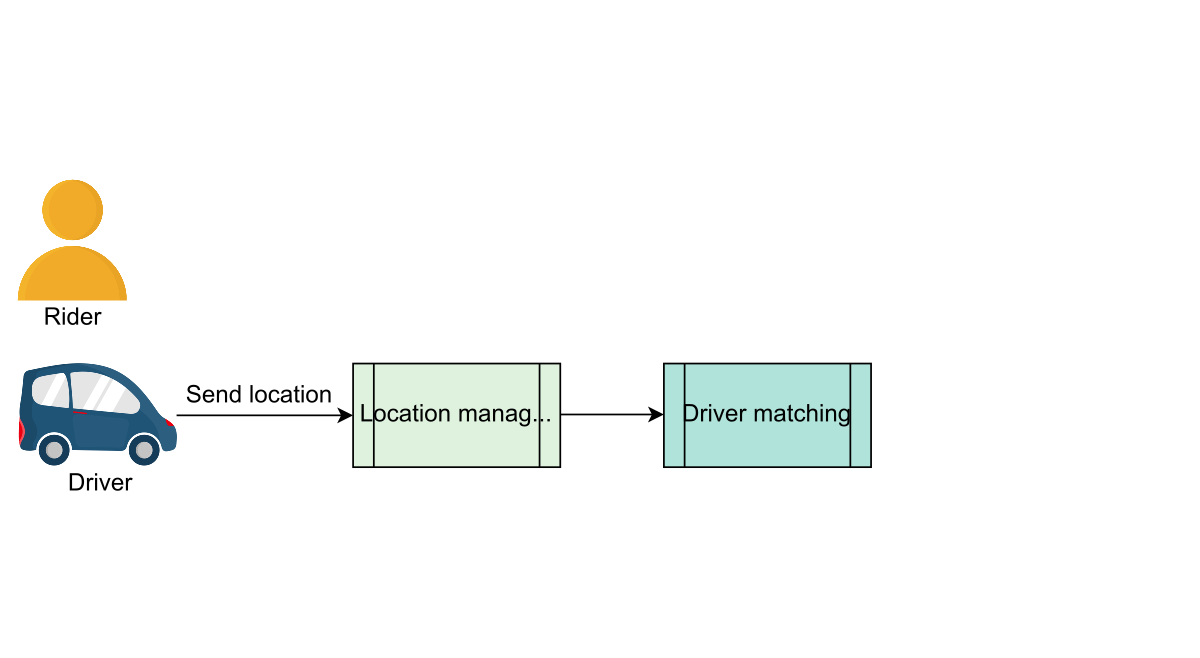
\includegraphics[width=\textwidth]{Images/chapter_30/section_5429357153091584/4863852969984000.png}
 \caption{The rider is yet to open the application. The driver constantly updates their location}
 \end{subfigure}
 \hfill
 \begin{subfigure}[b]{0.48\textwidth}
 \centering
 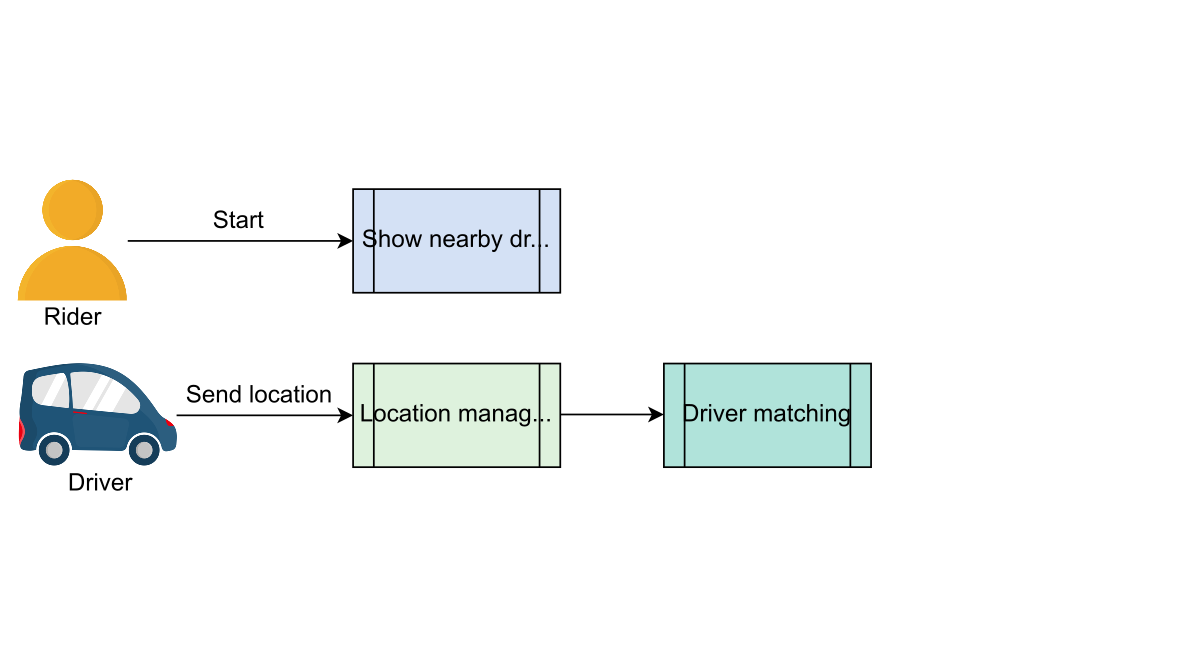
\includegraphics[width=\textwidth]{Images/chapter_30/section_5429357153091584/4780090101858304.png}
 \caption{The rider can see the nearby drivers when they open the application}
 \end{subfigure}
\end{figure}

\begin{figure}[htbp]
 \centering
 \begin{subfigure}[b]{0.48\textwidth}
 \centering
 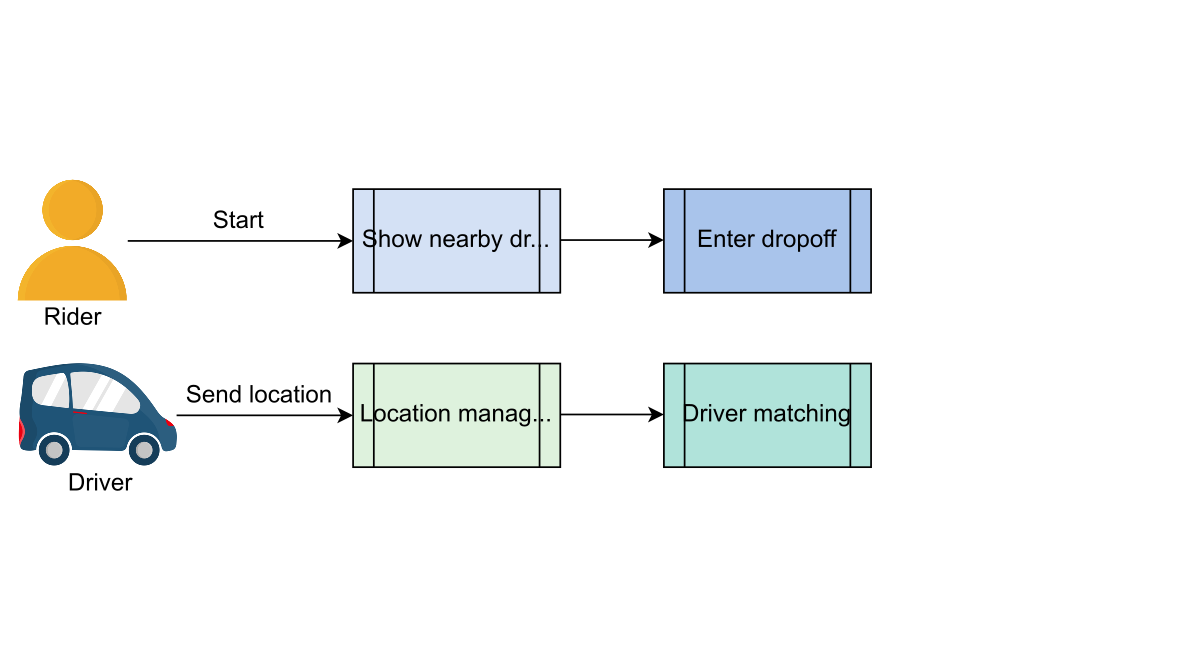
\includegraphics[width=\textwidth]{Images/chapter_30/section_5429357153091584/5120066895216640.png}
 \caption{The rider enters the drop-off location}
 \end{subfigure}
 \hfill
 \begin{subfigure}[b]{0.48\textwidth}
 \centering
 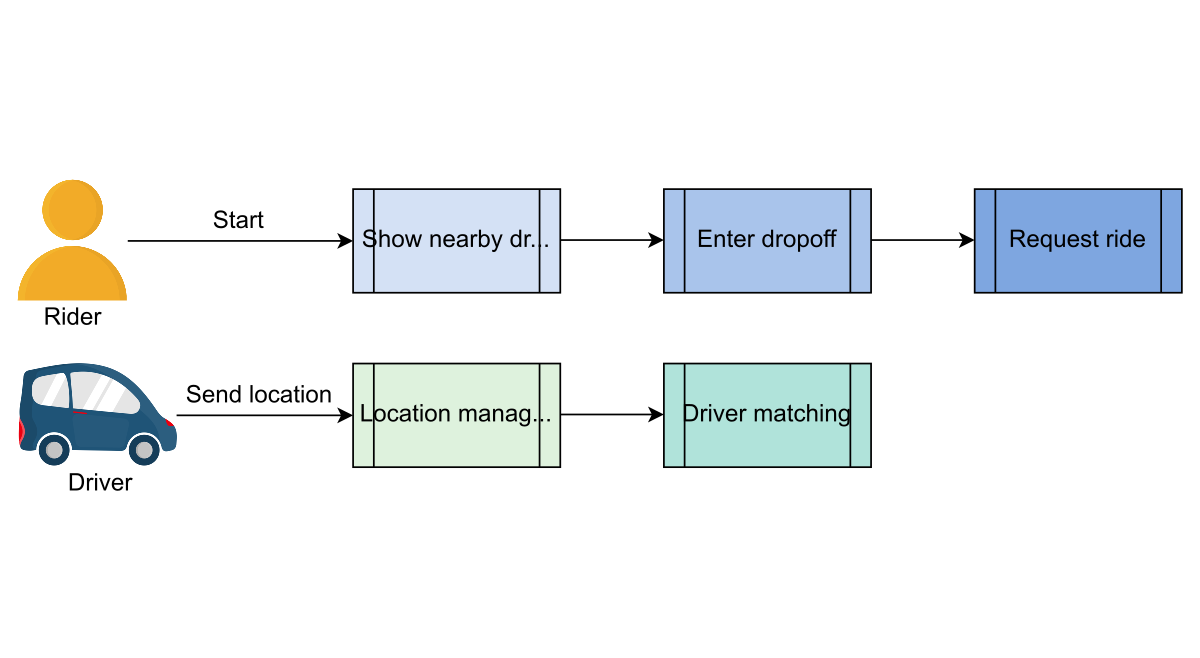
\includegraphics[width=\textwidth]{Images/chapter_30/section_5429357153091584/4504955167965184.png}
 \caption{The rider requests the ride}
 \end{subfigure}
\end{figure}

\begin{figure}[htbp]
 \centering
 \begin{subfigure}[b]{0.48\textwidth}
 \centering
 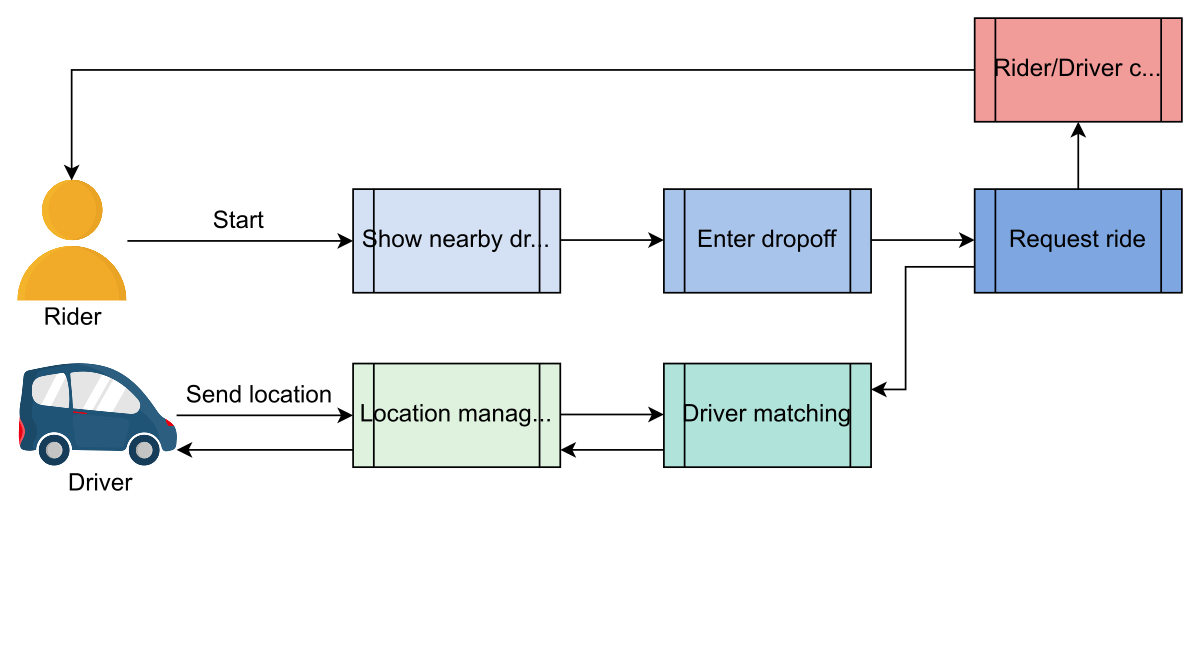
\includegraphics[width=\textwidth]{Images/chapter_30/section_5429357153091584/4806466905309184.png}
 \caption{The driver receives the request. The rider or driver can cancel the request here}
 \end{subfigure}
 \hfill
 \begin{subfigure}[b]{0.48\textwidth}
 \centering
 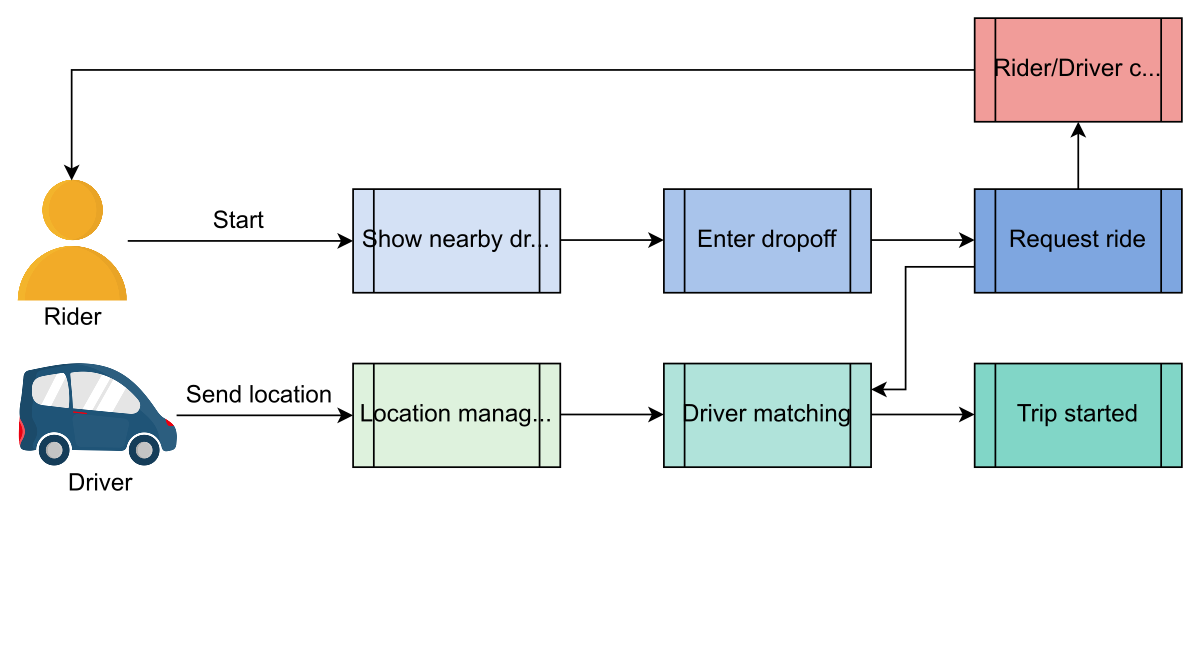
\includegraphics[width=\textwidth]{Images/chapter_30/section_5429357153091584/4663547842002944.png}
 \caption{The driver accepts the request and starts the trip}
 \end{subfigure}
\end{figure}

\begin{figure}[htbp]
 \centering
 \begin{subfigure}[b]{0.48\textwidth}
 \centering
 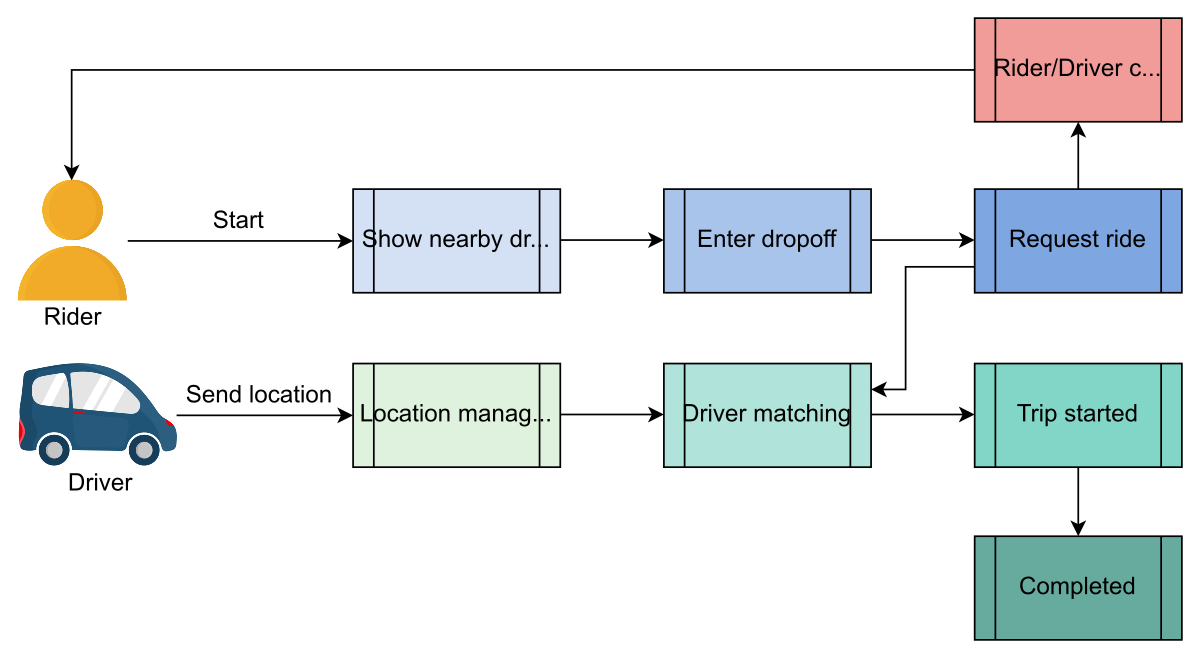
\includegraphics[width=\textwidth]{Images/chapter_30/section_5429357153091584/5495294330667008.png}
 \caption{The trip is completed}
 \end{subfigure}
\end{figure}

\subsection{High-level design of Uber}\label{hNX7_iXIMbsAMseEI359Q}
\\
At a high level, our system should be able to take requests for a ride from the rider and return the matched driver information and trip information to the rider. It also regularly takes the driver's location. Additionally , it returns the trip and rider information to the driver when the driver is matched to a rider.\\

\begin{figure}[htbp]
 \centering
 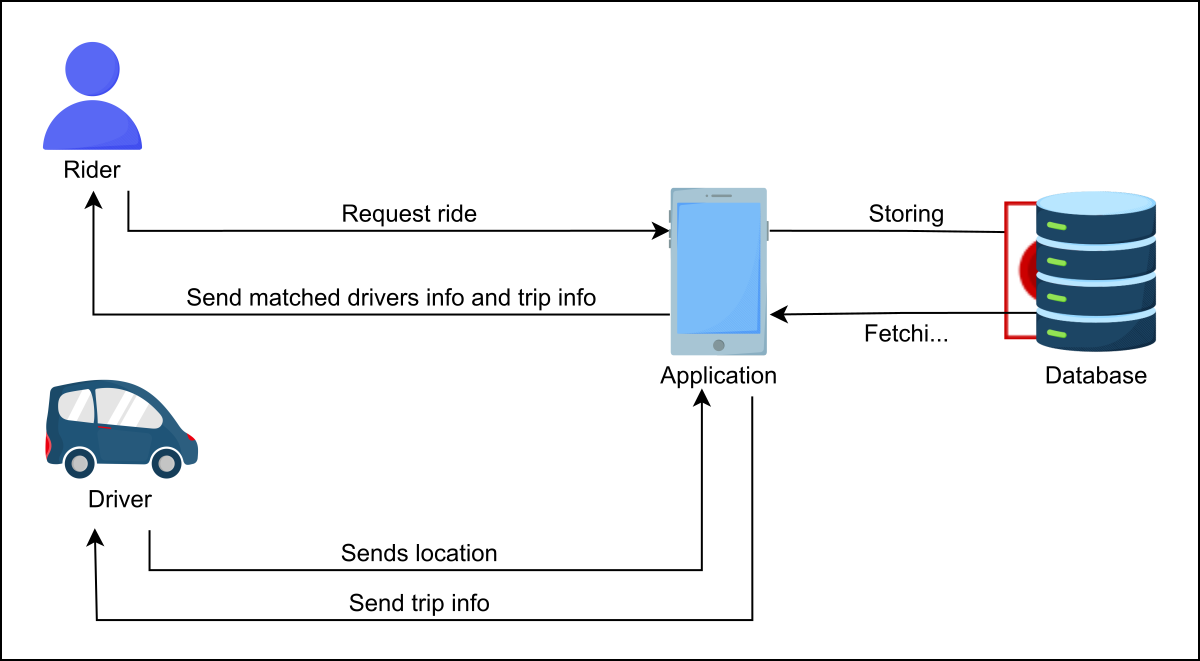
\includegraphics[width=0.5\textwidth]{Images/chapter_30/section_5429357153091584/5279089059823616.png}
 \caption{High-level design of Uber}
\end{figure}

\subsection{API design}\label{vk0fiix-6tZkNPxL0TIs5}
\\
Let's discuss the design of APIs according to the functionalities we provide. We 'll design APIs to translate our feature set into technical specifications.
\\
We won't repeat the description of repeating parameters in the following APIs.

\subsubsection{Update driver location}\label{mwhIKD_U9PZpVfK1heJNH}

\begin{lstlisting}[language=JavaScript]
updateDriverLocation(driverID, oldlat, oldlong, newlat, newlong )
\end{lstlisting}

\begin{table}[htbp]
\centering
\small
\adjustbox{max width=\textwidth}{
\begin{tabular}{|p{0.303\textwidth}|p{0.647\textwidth}|}
\hline
Parameter & Description \\
\hline
\hline
\texttt{driverID} & The ID of the driver \\
\hline
\texttt{oldlat} & The previous latitude of the driver \\
\hline
\texttt{oldlong} & The previous longitude of the driver \\
\hline
\texttt{newlat} & The new latitude of the driver \\
\hline
\texttt{newlong} & The new longitude of the driver \\
\hline
\end{tabular}
}
\end{table}

The \texttt{updateDriverLocation} API is used to send the driver's coordinates to the driver location servers. This is where the location of the driver is updated and communicated to the riders. Sending
\texttt{oldlat} and \texttt{oldlong} in the API call simplifies the server-side logic by reducing the need to fetch this data from the database. It also enables the service to track the actual route taken, even when the client couldn't send this data and was queuing locally. For clients with very low bandwidth, an alternate API without \texttt{oldlat} and \texttt{oldlong} can be used.

\subsubsection{Find nearby drivers}\label{gieXs3HGCYZye6Vuy5Sfs}

\begin{lstlisting}[language=JavaScript]
findNearbyDrivers(riderID, lat, long)
\end{lstlisting}

\begin{table}[htbp]
\centering
\small
\adjustbox{max width=\textwidth}{
\begin{tabular}{|p{0.303\textwidth}|p{0.647\textwidth}|}
\hline
Parameter & Description \\
\hline
\hline
\texttt{riderID} & The ID of the rider \\
\hline
\texttt{lat} & The latitude of the rider \\
\hline
\texttt{long} & The longitude of the rider \\
\hline
\end{tabular}
}
\end{table}

The \texttt{findNearbyDrivers} API is used to send the location of the rider for whom we want to find the nearby drivers.

\subsubsection{Request a ride}\label{eSMYA9XDvHpA4YKYbt4x5}

\begin{lstlisting}[language=JavaScript]
requestRide(riderID, lat, long, dropOfflat, dropOfflong, typeOfVehicle)
\end{lstlisting}

\begin{table}[htbp]
\centering
\small
\adjustbox{max width=\textwidth}{
\begin{tabular}{|p{0.303\textwidth}|p{0.647\textwidth}|}
\hline
Parameter & Description \\
\hline
\hline
\texttt{lat} & The current latitude of the rider \\
\hline
\texttt{long} & The current longitude of the rider \\
\hline
\texttt{dropOfflat} & The latitude of the rider's drop-off location \\
\hline
\texttt{dropOfflong}{\texttt{}} & The longitude of the rider's drop-off location \\
\hline
\texttt{typeOfVehicle} & The type of vehicle required by the rider---for example, business, economy, and so on. \\
\hline
\end{tabular}
}
\end{table}

The \texttt{requestRide} API is used to send the location of the rider and the type of vehicle the rider needs.

\subsubsection{Show driver ETA}\label{2Ar0IbtREsvUKEGumi2_x}

\begin{lstlisting}[language=JavaScript]
showETA(rider_lat, rider_lng, destination_lat, destination_lng, ride_type)
\end{lstlisting}

\begin{table}[htbp]
\centering
\small
\adjustbox{max width=\textwidth}{
\begin{tabular}{|p{0.303\textwidth}|p{0.647\textwidth}|}
\hline
Parameter & Description \\
\hline
\hline
\texttt{rider\_lat\ } & The latitude of the rider\textquotesingle s current location. \\
\hline
\texttt{rider\_lng} & The longitude of the rider\textquotesingle s current location. \\
\hline
\texttt{destination\_lat} & The latitude of the destination (optional, for trip ETA). \\
\hline
\texttt{destination\_lng} & The longitude of the destination (optional, for trip ETA). \\
\hline
\texttt{ride\_type} & The type of ride requested (e.g., "economy", "premium", "bike"). \\
\hline
\end{tabular}
}
\end{table}

The \texttt{showEta} API is used to show the estimated time of arrival to the rider.

\subsubsection{Confirm pickup}\label{qTWBuTPWHR7DQulA3jiFo}

\begin{lstlisting}[language=JavaScript]
confirmPickup(driverID, riderID, timestamp)
\end{lstlisting}

\begin{table}[htbp]
\centering
\small
\adjustbox{max width=\textwidth}{
\begin{tabular}{|p{0.303\textwidth}|p{0.647\textwidth}|}
\hline
Parameter & Description \\
\hline
\hline
\texttt{timestamp} & The time at which the driver picked up the rider \\
\hline
\end{tabular}
}
\end{table}

The \texttt{confirmPickup} API is used to determine when the driver has picked up the rider.

\subsubsection{Show trip updates}\label{B8-X44o_VDoD5G8j5uG56}

\begin{lstlisting}[language=JavaScript]
showTripUpdates(tripID, riderID, driverID, driverlat, driverlong, time_elapsed, time_remaining)
\end{lstlisting}

\begin{table}[htbp]
\centering
\small
\adjustbox{max width=\textwidth}{
\begin{tabular}{|p{0.303\textwidth}|p{0.647\textwidth}|}
\hline
Parameter & Description \\
\hline
\hline
\texttt{tripID} & The ID of the trip \\
\hline
\texttt{driverlat} & The latitude of the driver \\
\hline
\texttt{driverlong} & The longitude of the driver \\
\hline
\texttt{time\_elapsed}{\texttt{}} & The total time of the trip \\
\hline
\texttt{time\_remaining} & The time remaining (extract the current time from the ETA) to reach the destination \\
\hline
\end{tabular}
}
\end{table}

The \texttt{showTripUpdates} API is used to show the updates of the trip, including the position of the driver and the time remaining to reach the destination.

\subsubsection{End the trip}\label{nOuUyfeeuUbBbDhNsoOWb}

\begin{lstlisting}[language=JavaScript]
endTrip(tripID, riderID, driverID, time_elapsed, lat, long)
\end{lstlisting}

The \texttt{endTrip} API is used to end the trip.

% End of section content